\noindent WePlanner er en webapplikation som gør det nemmere for fællesskaber, at kunne kommunikere med hinanden. I den første udgave af webapplikationen, er der lagt fokus på at lave et fuldendt planlægningsværktøj for bofællesskaber og kollegier, og senere hen udvikle det til at kunne bruges i andre sociale sammenhænge.

En bruger opretter sig på hjemmesiden, og kan nu oprette en gruppe for sit fællesskab, eller blive inviteret via. E-mail, til en allerede eksisterende gruppe. Den bruger der opretter gruppen, er automatisk ejer af gruppen, og har dermed flere rettigheder end de andre brugere. Flere brugere kan godt blive gjort til administrator af gruppen.

Når gruppen er oprettet, kan brugere tilføje widgets til denne gruppe, som hver især har forskellige egenskaber. Når man er inde på gruppens forside, vises alle de tilføjede widgets med en overskrift, og den vigtigste information fra den enkelte widget. På denne måde kan man udefra gruppens forside, få et godt overblik af relevant information. Ved at klikke på en widget, udvides denne og al information kan findes heri.

\noindent De widgets der i første omgang skal udarbejdes er følgende:

\begin{itemize}
\item  \textbf{Kalender}

Her kan brugere tilføje begivenheder, som er relevant for de andre brugere i gruppen. Kalenderen kan bruges til at få et overblik over begivenheder for et fællesskab, eller en bruger.
\end{itemize}

\begin{itemize}
\item  \textbf{Pinned event}

Bruges til at fremhæve en begivenhed, hvis den er meget vigtig.
\end{itemize}


\begin{itemize}
\item  \textbf{Booking}

Her kan brugere gå ind og reservere ressourcer og se, hvornår en ressource er reserveret. Dette kan f.eks. bruges til at lave et bookingsystem af en fælles vaskemaskine.
\end{itemize}

\begin{itemize}
\item  \textbf{Planlægning}

Denne bruges til at lave planlægning over faste opgaver. Brugere kan gå ind og se, hvornår det er deres tur, og bytte deres vagter med de andre brugere. Dette kan f.eks. bruges til at lave en mad- eller rengøringsplan.
\end{itemize}

\begin{itemize}
\item  \textbf{Liste}

\noindent Kan bruges til at oprette en liste, som brugerne kan tilføje elementer til. Denne kan f.eks. bruges til at lave en fælles indkøbsliste.
\end{itemize}

\begin{itemize}
\item  \textbf{Betaling}

\noindent Her kan en bruger skrive ind, hvis han/hun har lagt ud for noget, som nogle af de andre brugere skal betale for. De betalende brugere går ind og markerer, når de har betalt, og den betalende bruger accepterer, at der er betalt tilbage.
\end{itemize}

\begin{itemize}
\item  \textbf{Opslagstavle}

\noindent Her kan brugere skrive et opslag, som kan være relevant for de andre brugere. Denne widget kan som den eneste deles med andre grupper. På den måde kan den fungere som en fælles opslagstavle for en hel opgang, uden at opgangen skal have en fælles gruppe.
\end{itemize}

\noindent Widgets som tilføjes, har hver deres indstillingsmuligheder, så de kan tilpasses efter gruppens behov. 

\subsection{Visualisering af produkt}
For at tydeliggøre, hvordan idéen visuelt ser ud, er der herunder lavet nogle udkast til at understøtte dette. Herunder på figur \ref{fig:login_site} er login-siden vist. Det er det første man, som bruger møder. Det er her muligt at logge ind med sin e-mail og password. Derudover er det også muligt at oprette en bruger, selvom dette ikke er vist.
\begin{figure}[H]
  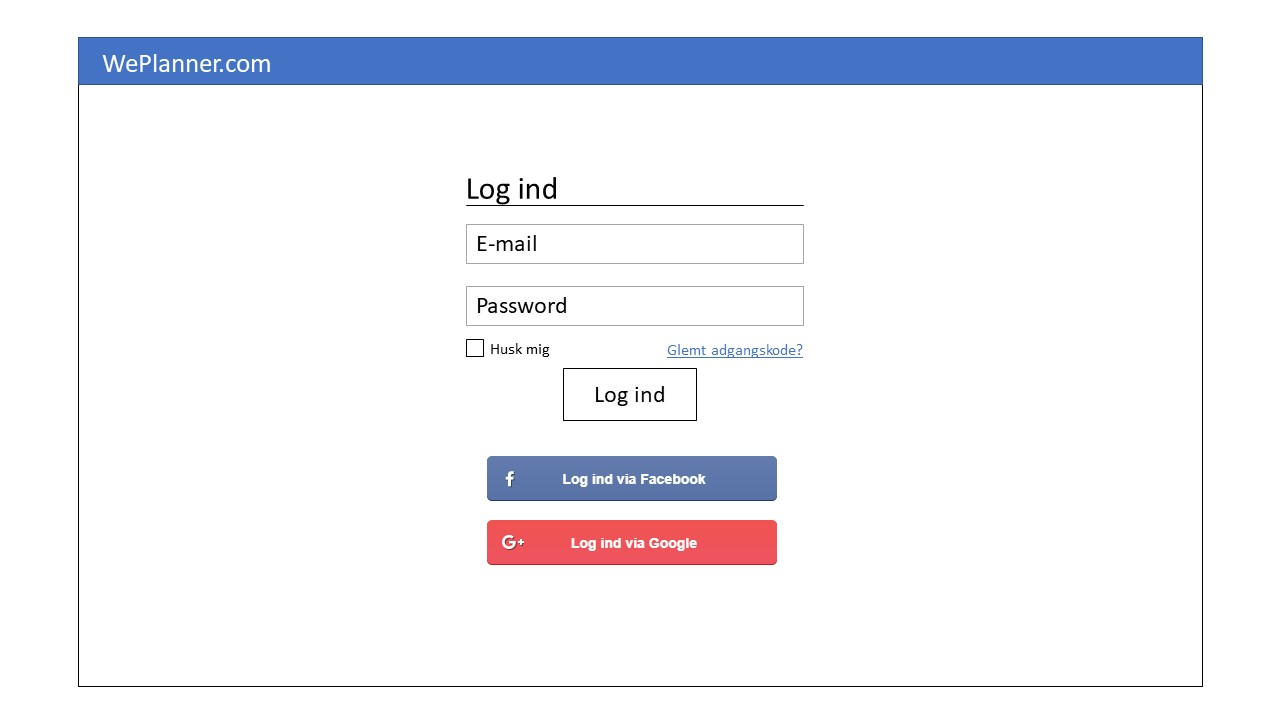
\includegraphics[width=\linewidth]{01_Billeder/04_Indledning/Slide1.JPG}
  \centering
  \caption{Login side}
  \label{fig:login_site}
\end{figure}

\noindent Når man er logget ind med sin bruger, møder man 'Home' siden, som kan ses på figur \ref{fig:home_site}. Her kan brugeren se alle de grupper, hvor brugeren er medlem. Derudover har brugeren også mulighed for at oprette en gruppe.
\begin{figure}[H]
  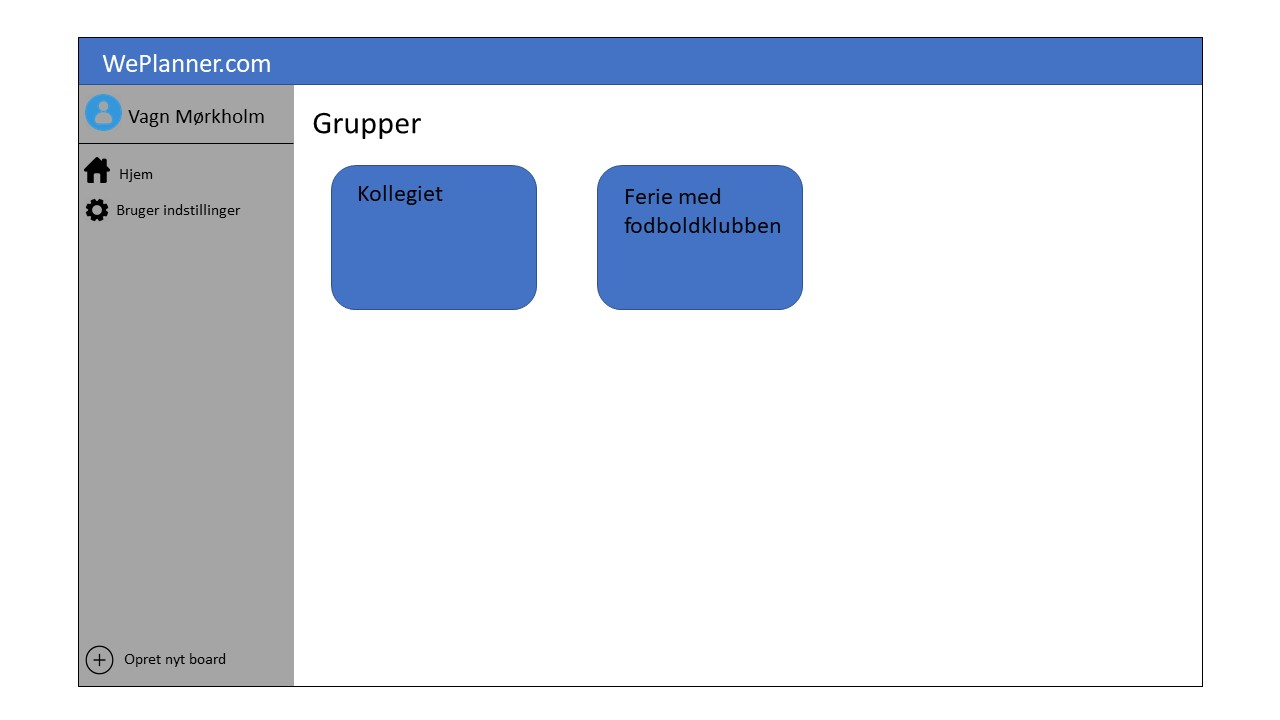
\includegraphics[width=\linewidth]{01_Billeder/04_Indledning/Slide2.JPG}
  \centering
  \caption{Home side}
  \label{fig:home_site}
\end{figure}

\noindent Ved at vælge en gruppe, kommer man ind på en ny side, som viser gruppens widgets. Her kan brugeren få et hurtigt overblik ved at kigge på de forskellige widgets. Brugeren kan så trykke på en widget, for at få vist flere informationer. Dette ses på figur \ref{fig:board_site}.
\begin{figure}[H]
  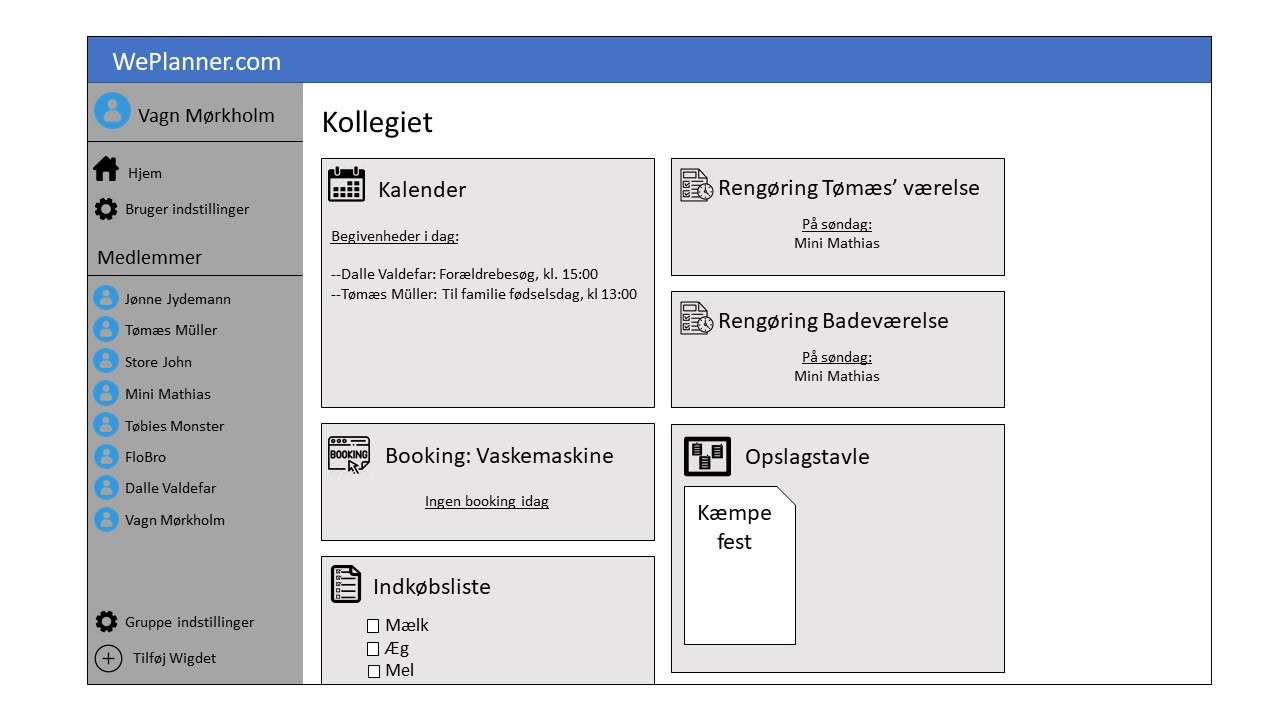
\includegraphics[width=\linewidth]{01_Billeder/04_Indledning/Slide3.JPG}
  \centering
  \caption{Gruppeside}
  \label{fig:board_site}
\end{figure}

